\documentclass[11pt]{article}
% Adapted from an original template by Hlyni Arnórssyni,
% Reykjavik University, Iceland

% ------------------------------ PAGE SETTINGS ------------------------------
\usepackage{geometry}

\geometry{
    paper=a4paper,
    top=2.5cm,
    bottom=2.5cm,
    left=2.5cm,
    right=2.4cm,
    headheight=0.75cm,
    footskip=1.5cm,
    headsep=0.75cm
}

% ------------------------------ BASIC PACKAGES ------------------------------
\usepackage{blindtext}

% Character encoding
\usepackage[T1]{fontenc}
\usepackage[utf8]{inputenc}

% Mathematics
\usepackage{amsmath, amsfonts, amsthm, amssymb}
\usepackage{braket, nicefrac}

% SI units
\usepackage{siunitx}

% Lists / columns
\usepackage{enumitem, multicol}

% ------------------------------ FIGURES ------------------------------
\usepackage{graphicx}
\usepackage{float}
\usepackage{keystroke}
\usepackage{pgfplots}
\usepgfplotslibrary{units}
\pgfplotsset{compat=1.16}

% Search these locations automatically for figures
\graphicspath{{fig/}{graphics/}{Graphics/}{./}}

% ------------------------------ TABLES ------------------------------
\usepackage{tabularx}
\usepackage{array}
\usepackage[table]{xcolor}

% ------------------------------ TYPOGRAPHY ------------------------------
\usepackage{caption}
\usepackage{titlesec}
\usepackage{microtype}
\usepackage{csquotes}

% ------------------------------ COLORS ------------------------------
\definecolor{GWBlue}{HTML}{1E4E79}

% ------------------------------ SECTION STYLING ------------------------------
\titleformat{\section}
  {\Large\bfseries\color{GWBlue}}
  {\thesection.}
  {0.40em}
  {}

\titlespacing*{\section}
  {0pt}
  {0.70em}
  {0.28em}

% ------------------------------ CAPTION STYLING ------------------------------
\captionsetup{
    font=small,
    labelfont=bf,
    textfont=it,
    labelsep=period,
    skip=4pt
}

% ------------------------------ PARAGRAPH SPACING ------------------------------
\setlength{\parindent}{0pt}
\setlength{\parskip}{0.30em}

% ------------------------------ BIBLIOGRAPHY ------------------------------
\usepackage[
    backend=biber,
    style=authoryear,
    sorting=none,
    giveninits=true,
    maxbibnames=99,
    dashed=false
]{biblatex}

\addbibresource{references.bib}

\DeclareNameAlias{sortname}{family-given}
\DeclareNameAlias{default}{family-given}
\DeclareFieldFormat[article]{title}{#1}
\DeclareFieldFormat[misc]{title}{#1}
\renewbibmacro{in:}{}

\AtEveryBibitem{%
    \clearfield{doi}%
    \clearfield{urldate}%
}

\AtBeginBibliography{\small}
\setlength{\bibitemsep}{0.35em}

% ------------------------------ HYPERLINKS ------------------------------
\usepackage{hyperref}

\hypersetup{
    colorlinks=true,
    linkcolor=GWBlue,
    citecolor=GWBlue,
    urlcolor=GWBlue
}

\begin{document}

\begin{titlepage}
\centering
\thispagestyle{empty}

\vspace*{0.15in}


\includegraphics[
    width=0.5\textwidth
]{gwu_logo.pdf}

\vspace{0.28in}

{\large\bfseries Data Science Program\par}
{\large\bfseries Department of Data Science\par}
{\large DATS 6501 - Capstone Project - Fall 2026\par}

\vspace{0.38in}

{\Large\bfseries
Post-Training Analysis \& Novelty Detection Using\par}

\vspace{0.08in}

{\Large\bfseries
Neural Network Self-Organizing Maps (NNSOM)\par}

\vspace{0.34in}

{\large\bfseries
PHASE 2 REPORT\par}

\vspace{0.22in}

{\large\bfseries
NNSOM Training, Cluster and Error Analysis\par}
\vspace{0.12in}
{\large\bfseries Fashion-MNIST\par}

\vspace{0.36in}

{\large\bfseries Capstone - Group 5\par}

\vspace{0.08in}

{\large\bfseries Fyrooz Anika Khan\par}
{\large\bfseries Nazish Atta\par}

\vspace{0.30in}

{\large The George Washington University\par}
{\large Washington, DC\par}

\vspace{0.30in}

{\large\itshape Supervised by\par}
{\large\itshape Dr. Amir Jafari\par}
{\large\itshape Associate Professor of Data Science\par}

\vspace*{\fill}

\end{titlepage}

\setcounter{page}{2}
\newcommand{\tbd}{\textbf{[TBD]}}
\setlength{\emergencystretch}{3em}

\section{SOM 15$\times$15 Overview}

This phase applies the MNIST 15$\times$15 Self-Organizing Map (SOM) recipe, unchanged, to the 84-dimensional \texttt{fc2} embeddings of the Fashion-MNIST network from Phase 1 \cite{kohonen1990som,jafari_nnsom,xiao2017fashion}. The map is trained on the 49,000 training embeddings and examined on the 10,500 validation embeddings. On Fashion-MNIST the network makes 876 validation mistakes (against 92 on MNIST), so this is a much stronger test of whether the map shows where the network fails.

\textbf{Summary of the results.}
\begin{itemize}[leftmargin=1.4em, itemsep=1pt]
  \item \textbf{The map trained well.} 225 of 225 cells receive training images and 222 receive validation images. Training and validation images fit the map equally well (quantization error 0.915 and 0.899).
  \item \textbf{The classes form regions, but less cleanly than on MNIST.} 89.3\% of the validation images sit in a cell whose most common class is their own class (MNIST: 98.2\%). With shuffled labels this would be only 17.3\%. The mixed cells lie in the part of the map that holds the upper-body garments.
  \item \textbf{The mistakes gather in a few cells.} The 11 hotspot cells (5\% of the map) hold 3.9 times their fair share of the mistakes, tested on images not used to pick them (chance: about 1.0). The same holds on 10$\times$10 and 20$\times$20 maps.
  \item \textbf{Mistakes sit where classes mix,} even more strongly than on MNIST: the Spearman correlation between a cell's error rate and its purity is $-0.95$ (MNIST: $-0.81$).
  \item \textbf{The \texttt{fc2} layer is the better layer for the map.} SOMs on \texttt{fc2} find the network's mistakes better and have purer cells than SOMs on the earlier \texttt{fc1} layer, in all 5 SOM seeds (Section~\ref{sec:ablation}).
  \item \textbf{15$\times$15 is a good grid.} In the fair comparison fixed in advance, its cells predict the network's mistakes better than a 20$\times$20 map's (AUROC difference $-0.042$ for 20$\times$20) and as well as a 10$\times$10 map's.
  \item \textbf{But the SOM is not the best mistake finder.} A k-means grouping finds mistakes as well as the SOM cells (AUROC 0.812 against 0.811), and the network's own confidence does better (0.906). As on MNIST, the SOM's value is the picture it gives of \emph{where} the mistakes are.
\end{itemize}

\subsection*{Where each item of the plan is covered}

{\small
\renewcommand{\arraystretch}{1.12}
\begin{tabularx}{\textwidth}{|>{\raggedright\arraybackslash}p{0.52\textwidth}|X|}
\hline
\textbf{What Phase 2 asks for} & \textbf{Where} \\ \hline
Set up NNSOM, grid size and training settings & Section~\ref{sec:training}, Tables~\ref{tab:grids} and~\ref{tab:gridcmp}, Figure~\ref{fig:gridcmp} \\ \hline
Train on training embeddings, monitor quantization error per epoch & Figure~\ref{fig:qe} \\ \hline
Component planes, hit histogram, U-matrix & Figures~\ref{fig:umatrix} and~\ref{fig:planes} \\ \hline
Assign each image to its best-matching cell; purity and class--cell intersection & Section~\ref{sec:cluster}, Figure~\ref{fig:purity} \\ \hline
Confusions overlaid on the map & Figure~\ref{fig:overlay} \\ \hline
Correct against misclassified images on the map; error hotspots & Section~\ref{sec:error}, Tables~\ref{tab:hotspots} and~\ref{tab:robust}, Figure~\ref{fig:errormaps} \\ \hline
Which network layer to map (feature-layer ablation) & Section~\ref{sec:ablation}, Table~\ref{tab:ablation} \\ \hline
Images in the hotspots, and why they are hard & Section~\ref{sec:error}, Table~\ref{tab:hotspots}, Figure~\ref{fig:samples} \\ \hline
Comparison with simple baselines & Table~\ref{tab:baselines} \\ \hline
\end{tabularx}}

\section{Key terms in plain words}

{\small
\renewcommand{\arraystretch}{1.12}
\begin{tabularx}{\textwidth}{|>{\raggedright\arraybackslash}p{0.24\textwidth}|X|}
\hline
\textbf{Term} & \textbf{What it means} \\ \hline
Embedding (fc2) & The 84 numbers the CNN computes for an image just before it gives its answer. The SOM is trained on these numbers, not on the pixels. \\ \hline
SOM, cell (neuron) & A grid of cells, each holding a weight vector of 84 numbers. After training, similar images land in the same or nearby cells. \\ \hline
Best-matching unit (BMU) & The cell whose weights are closest to an image's embedding. Every image is assigned to its BMU. \\ \hline
Neighbourhood radius & How far on the grid the winning cell's ``pull'' reaches during training. It starts large (so the map orders itself) and shrinks to 1 (so it fits the data). \\ \hline
Quantization error (QE) & The average distance between an image and its BMU. Lower means the map fits the data more closely. \\ \hline
Topological error (TE1) & The share of images whose two closest cells are not next to each other on the grid. Lower means a better ordered map. \\ \hline
Hit histogram, U-matrix & How many images land in each cell; and the distance between each cell and its neighbours (high values mark borders between groups of cells). \\ \hline
Component plane & One map per embedding number, showing where on the grid that number is high or low. \\ \hline
Purity, entropy & Purity is the share of a cell's images that belong to its most common class. Entropy measures how mixed the classes in a cell are (0 means one class only). \\ \hline
Label shuffle (null) & The same measure recomputed after mixing up the labels at random. It shows what ``by chance'' would look like. \\ \hline
Hotspot, Wilson lower bound & A hotspot is a cell where the CNN makes many more mistakes than average. Cells are ranked by a cautious estimate of their error rate (the Wilson lower bound \cite{wilson1927probable}), so a small cell does not rank high by luck. \\ \hline
Concentration ratio & The hotspots' share of mistakes divided by their share of images. A ratio of 1 means the mistakes are spread evenly. \\ \hline
\end{tabularx}}

\section{SOM Training}\label{sec:training}

\begin{itemize}[leftmargin=1.4em, itemsep=2pt]
\item \textbf{Set-up (same as MNIST, fixed before any Fashion-MNIST data was loaded).} The SOM is trained with NNSOM's batch rule \cite{jafari_nnsom} on the 49,000 training embeddings, rescaled to $-1$ to $1$ with a scaler fitted on the training embeddings only. Hexagonal 15$\times$15 grid (225 cells), 250 epochs, neighbourhood radius shrinking from 11 to 1, seed 42. Run ID \texttt{som\_15x15\_nb11\_ep250\_s42}. The batch rule has no learning rate; the shrinking radius plays that role.

\item \textbf{Grid sizes (Table~\ref{tab:grids}).} The 10$\times$10 (radius 7) and 20$\times$20 (radius 15) maps were trained with the same recipe as checks. As on MNIST, a larger grid fits the data more closely (lower QE) but has a higher topological error. These single maps are descriptive; the protocol fixed 15$\times$15 as the headline map in advance and tested that choice with the fair comparison below.

\item \textbf{Fair grid comparison (Table~\ref{tab:gridcmp}, Figure~\ref{fig:gridcmp}).} MNIST's pre-registered design, unchanged. Each grid tried three starting radii and kept the best by QE and topological error, without labels (it kept 7, 11 and 15, the settings above). Each grid then trained 10 maps on resampled training data. The test: work out each cell's error rate on one half of the validation images and use it to predict the network's mistakes on the other half (AUROC), over 200 random splits. The rule, fixed in advance: if the whole 95\% range of a difference lies on one side of 0, one grid is better; if it lies inside $\pm0.02$, they are the same; otherwise inconclusive. \textbf{The primary comparison is decided: 15$\times$15 is better than 20$\times$20} ($-0.042$ for 20$\times$20, range $-0.077$ to $-0.008$). 15$\times$15 and 10$\times$10 cannot be told apart. As on MNIST, a bigger map is sharper (lower QE, purer cells) but no better at finding mistakes; here it is worse, probably because each of its cells holds fewer images, so its error rates are noisier. On MNIST the same test was inconclusive, because 92 mistakes were too few; with 876 mistakes the ranges are about three times narrower.

\item \textbf{Optuna check of the settings.} As in the protocol, 20 Optuna trials per grid searched the starting radius and the number of epochs, and the setting found was checked against the fixed one with 5 SOM seeds. On 15$\times$15, Optuna's setting (radius 7, 200 epochs) lowers QE slightly ($-0.014$, 95\% interval $-0.024$ to $-0.004$) but raises TE1 clearly ($+2.4$ points, $+1.6$ to $+3.2$). On no grid was Optuna's setting better on both measures, so the headline map stays as fixed.

\item \textbf{The chosen map.} QE is 0.915 on training images and 0.899 on validation images; TE1 is 5.30\% and 5.37\%. All 225 cells receive training images (at most 595 per cell); 3 cells receive no validation image. Training and validation numbers are almost the same, so the map describes new images as well as the ones it was trained on.

\item \textbf{Training curve (Figure~\ref{fig:qe}).} The QE drops from 3.06 to below 1 within the first few epochs, rises a little (to about 1.05--1.15) while the shrinking radius keeps reorganising the map, and settles at 0.915 in the last epochs, when the radius is close to 1. The curve is flat at the end, so 250 epochs are enough.

\item \textbf{Map pictures (Figures~\ref{fig:umatrix} and~\ref{fig:planes}).} Images are spread over the whole map. The footwear classes (sandals, sneakers, ankle boots) sit on the left of the map, and the U-matrix shows its strongest, dark-red borders around that side. Inside the clothing part, in the middle and right of the map, the borders are much weaker, which already hints that those classes overlap.
\end{itemize}

\begin{table}[H]
\centering
\renewcommand{\arraystretch}{1.12}
\small
\begin{tabular}{|l|c|c|c|}
\hline
\textbf{Measure (validation, one map each, seed 42)} & \textbf{10$\times$10} & \textbf{15$\times$15} & \textbf{20$\times$20} \\ \hline
Starting neighbourhood radius & 7 & 11 & 15 \\ \hline
Quantization error (QE) & 1.008 & 0.899 & 0.822 \\ \hline
Topological error TE1 (\%) & 4.26 & 5.37 & 7.33 \\ \hline
Topological error TE1+2 (\%) & 1.76 & 3.55 & 4.75 \\ \hline
Cells used, validation (\%) & 99.0 & 98.7 & 99.0 \\ \hline
\end{tabular}
\caption{The three grid sizes, with the MNIST recipe. Descriptive only; the headline grid was fixed in advance.}
\label{tab:grids}
\end{table}

\begin{table}[H]
\centering
\renewcommand{\arraystretch}{1.12}
\footnotesize\setlength{\tabcolsep}{3pt}
\begin{tabular}{|l|c|c|c|}
\hline
\textbf{Per grid (mean of 10 maps)} & \textbf{10$\times$10} & \textbf{15$\times$15} & \textbf{20$\times$20} \\ \hline
AUROC, held-out mistakes [95\% range] & 0.806 [0.780, 0.830] & 0.786 [0.757, 0.812] & 0.744 [0.714, 0.775] \\ \hline
AUROC for the 525 least-confident images & 0.864 & 0.843 & 0.796 \\ \hline
QE / TE1 (\%) & 1.054 / 4.84 & 0.913 / 6.26 & 0.844 / 7.66 \\ \hline
Purity (\%) & 87.9 & 89.0 & 89.5 \\ \hline
\multicolumn{4}{|l|}{\textbf{Differences} (bigger grid minus smaller, AUROC for mistakes)} \\ \hline
20$\times$20 $-$ 15$\times$15 (primary) & \multicolumn{3}{c|}{$-0.042$ [$-0.077$, $-0.008$]: \textbf{15$\times$15 better}} \\ \hline
15$\times$15 $-$ 10$\times$10 & \multicolumn{3}{c|}{$-0.019$ [$-0.054$, $+0.009$]: inconclusive} \\ \hline
20$\times$20 $-$ 10$\times$10 (exploratory) & \multicolumn{3}{c|}{$-0.061$ [$-0.100$, $-0.020$]: 10$\times$10 better} \\ \hline
\end{tabular}
\caption{Fair grid comparison: 10 maps per grid, 200 random half-splits of the 876 validation mistakes. The 20$\times$20 minus 10$\times$10 row was added after the MNIST result was known and is not part of the decision. The secondary measures (average precision, least-confident images) for 20$\times$20 against 15$\times$15 are all inconclusive. Run \texttt{grid\_comparison\_g10\_15\_20\_b10\_r200}.}
\label{tab:gridcmp}
\end{table}

\begin{figure}[H]
\centering
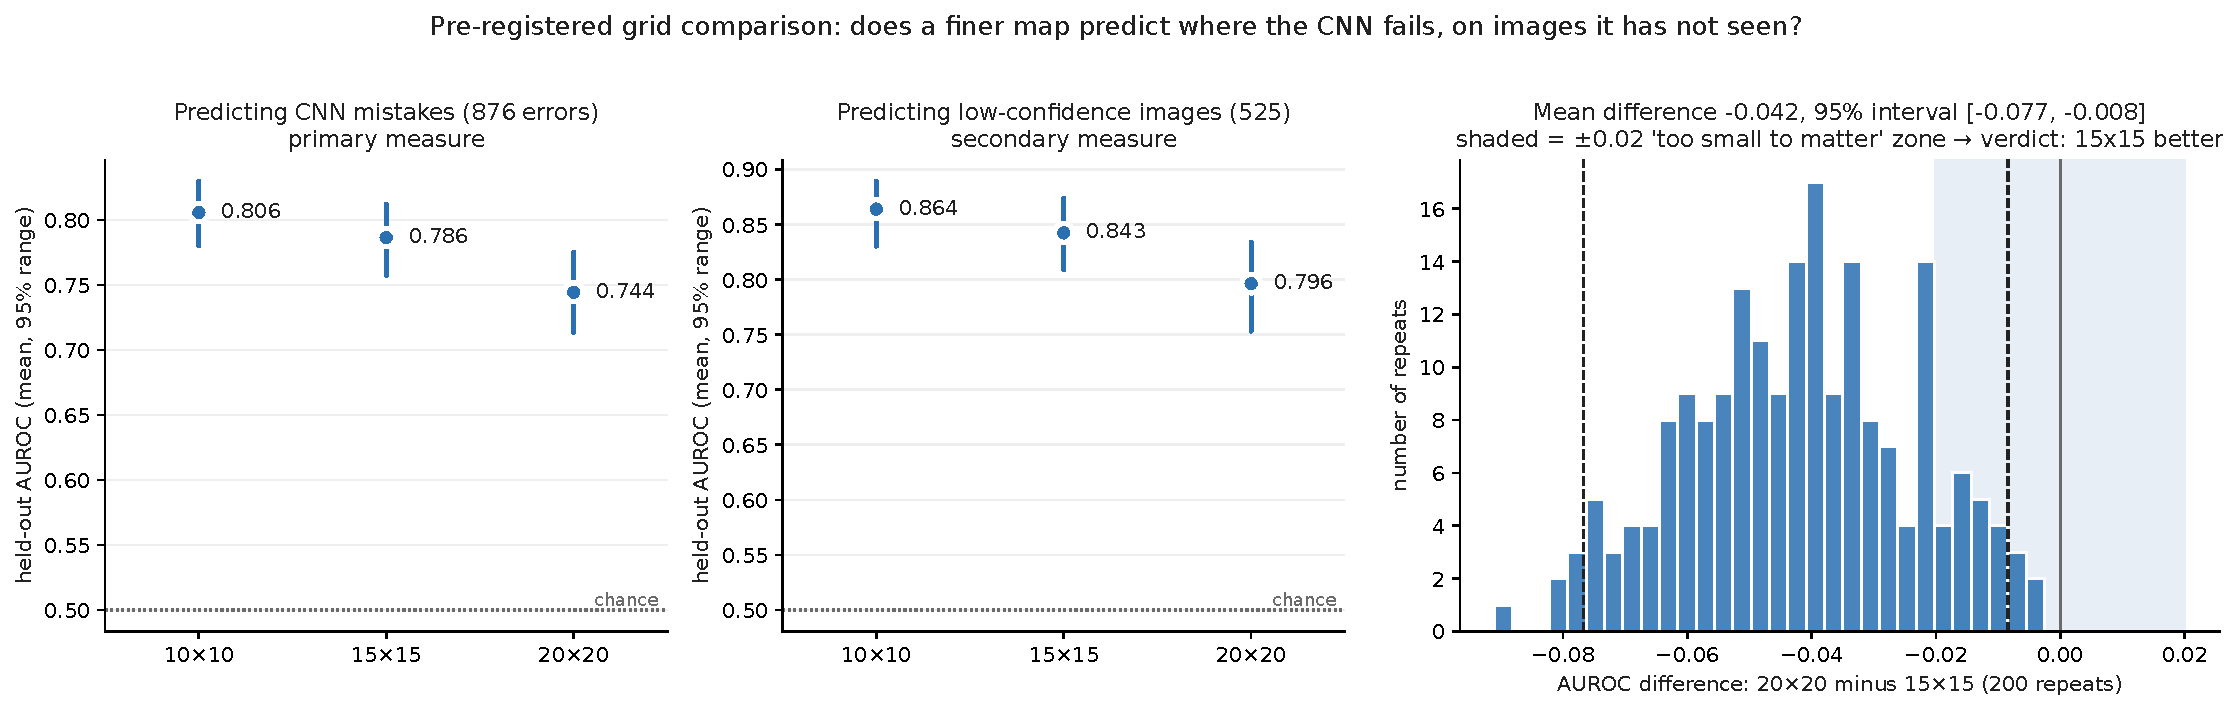
\includegraphics[width=\textwidth]{fig/som_nnsom_training/grid_comparison/grid_comparison_results.pdf}
\caption{Fair grid comparison. Left and middle: held-out AUROC per grid for the network's mistakes and for the least-confident images (mean and 95\% range). Right: the 200 differences between 20$\times$20 and 15$\times$15; the range lies below 0, so 15$\times$15 is better.}
\label{fig:gridcmp}
\end{figure}

\begin{figure}[H]
\centering
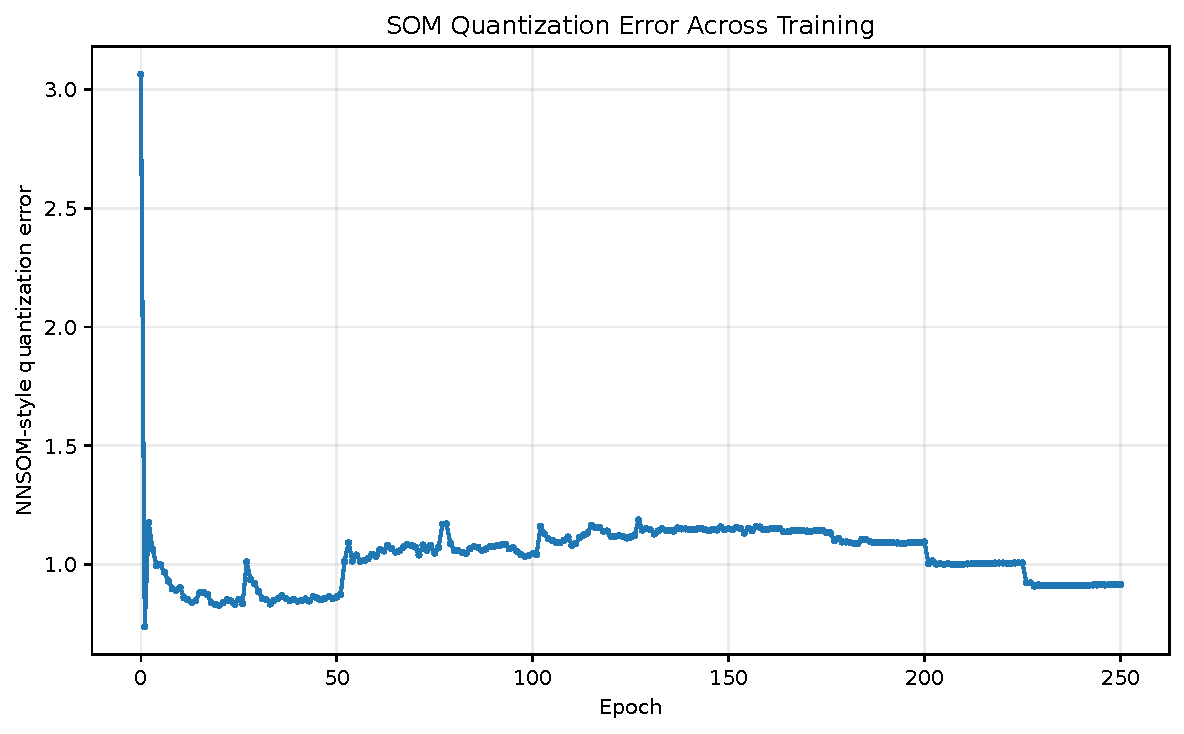
\includegraphics[width=0.62\textwidth]{fig/som_nnsom_training/convergence/som_15x15_nb11_ep250_s42_qe_curve.pdf}
\caption{Quantization error of the 15$\times$15 map on the training images after each of the 250 epochs.}
\label{fig:qe}
\end{figure}

\begin{figure}[H]
\centering
\begin{minipage}[c]{0.48\textwidth}\centering
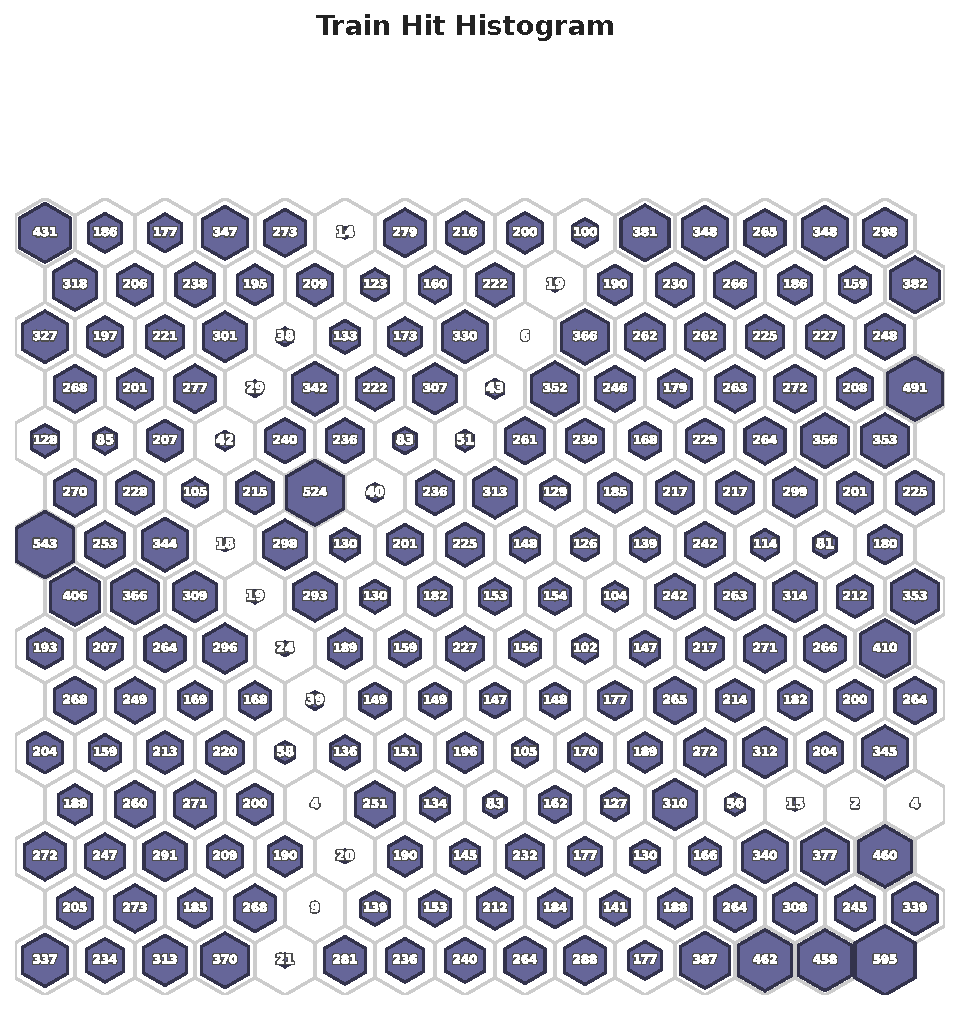
\includegraphics[width=\linewidth,keepaspectratio]{fig/som_nnsom_training/core/train_hit_histogram.pdf}
\end{minipage}\hfill
\begin{minipage}[c]{0.48\textwidth}\centering
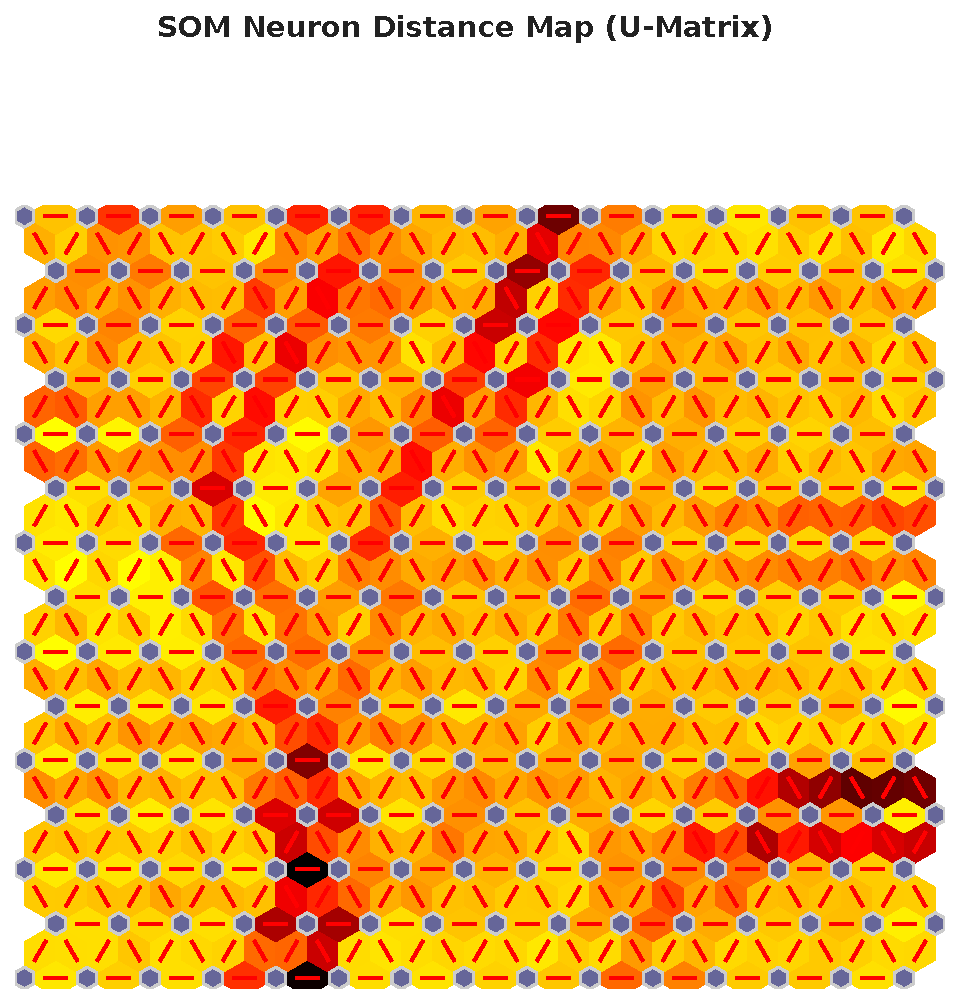
\includegraphics[width=\linewidth,keepaspectratio]{fig/som_nnsom_training/core/u_matrix_neuron_distance.pdf}
\end{minipage}
\caption{Left: hit histogram, the number of training images in each cell. Right: U-matrix, the distance between neighbouring cells (dark red: a border between groups of cells).}
\label{fig:umatrix}
\end{figure}

\begin{figure}[H]
\centering
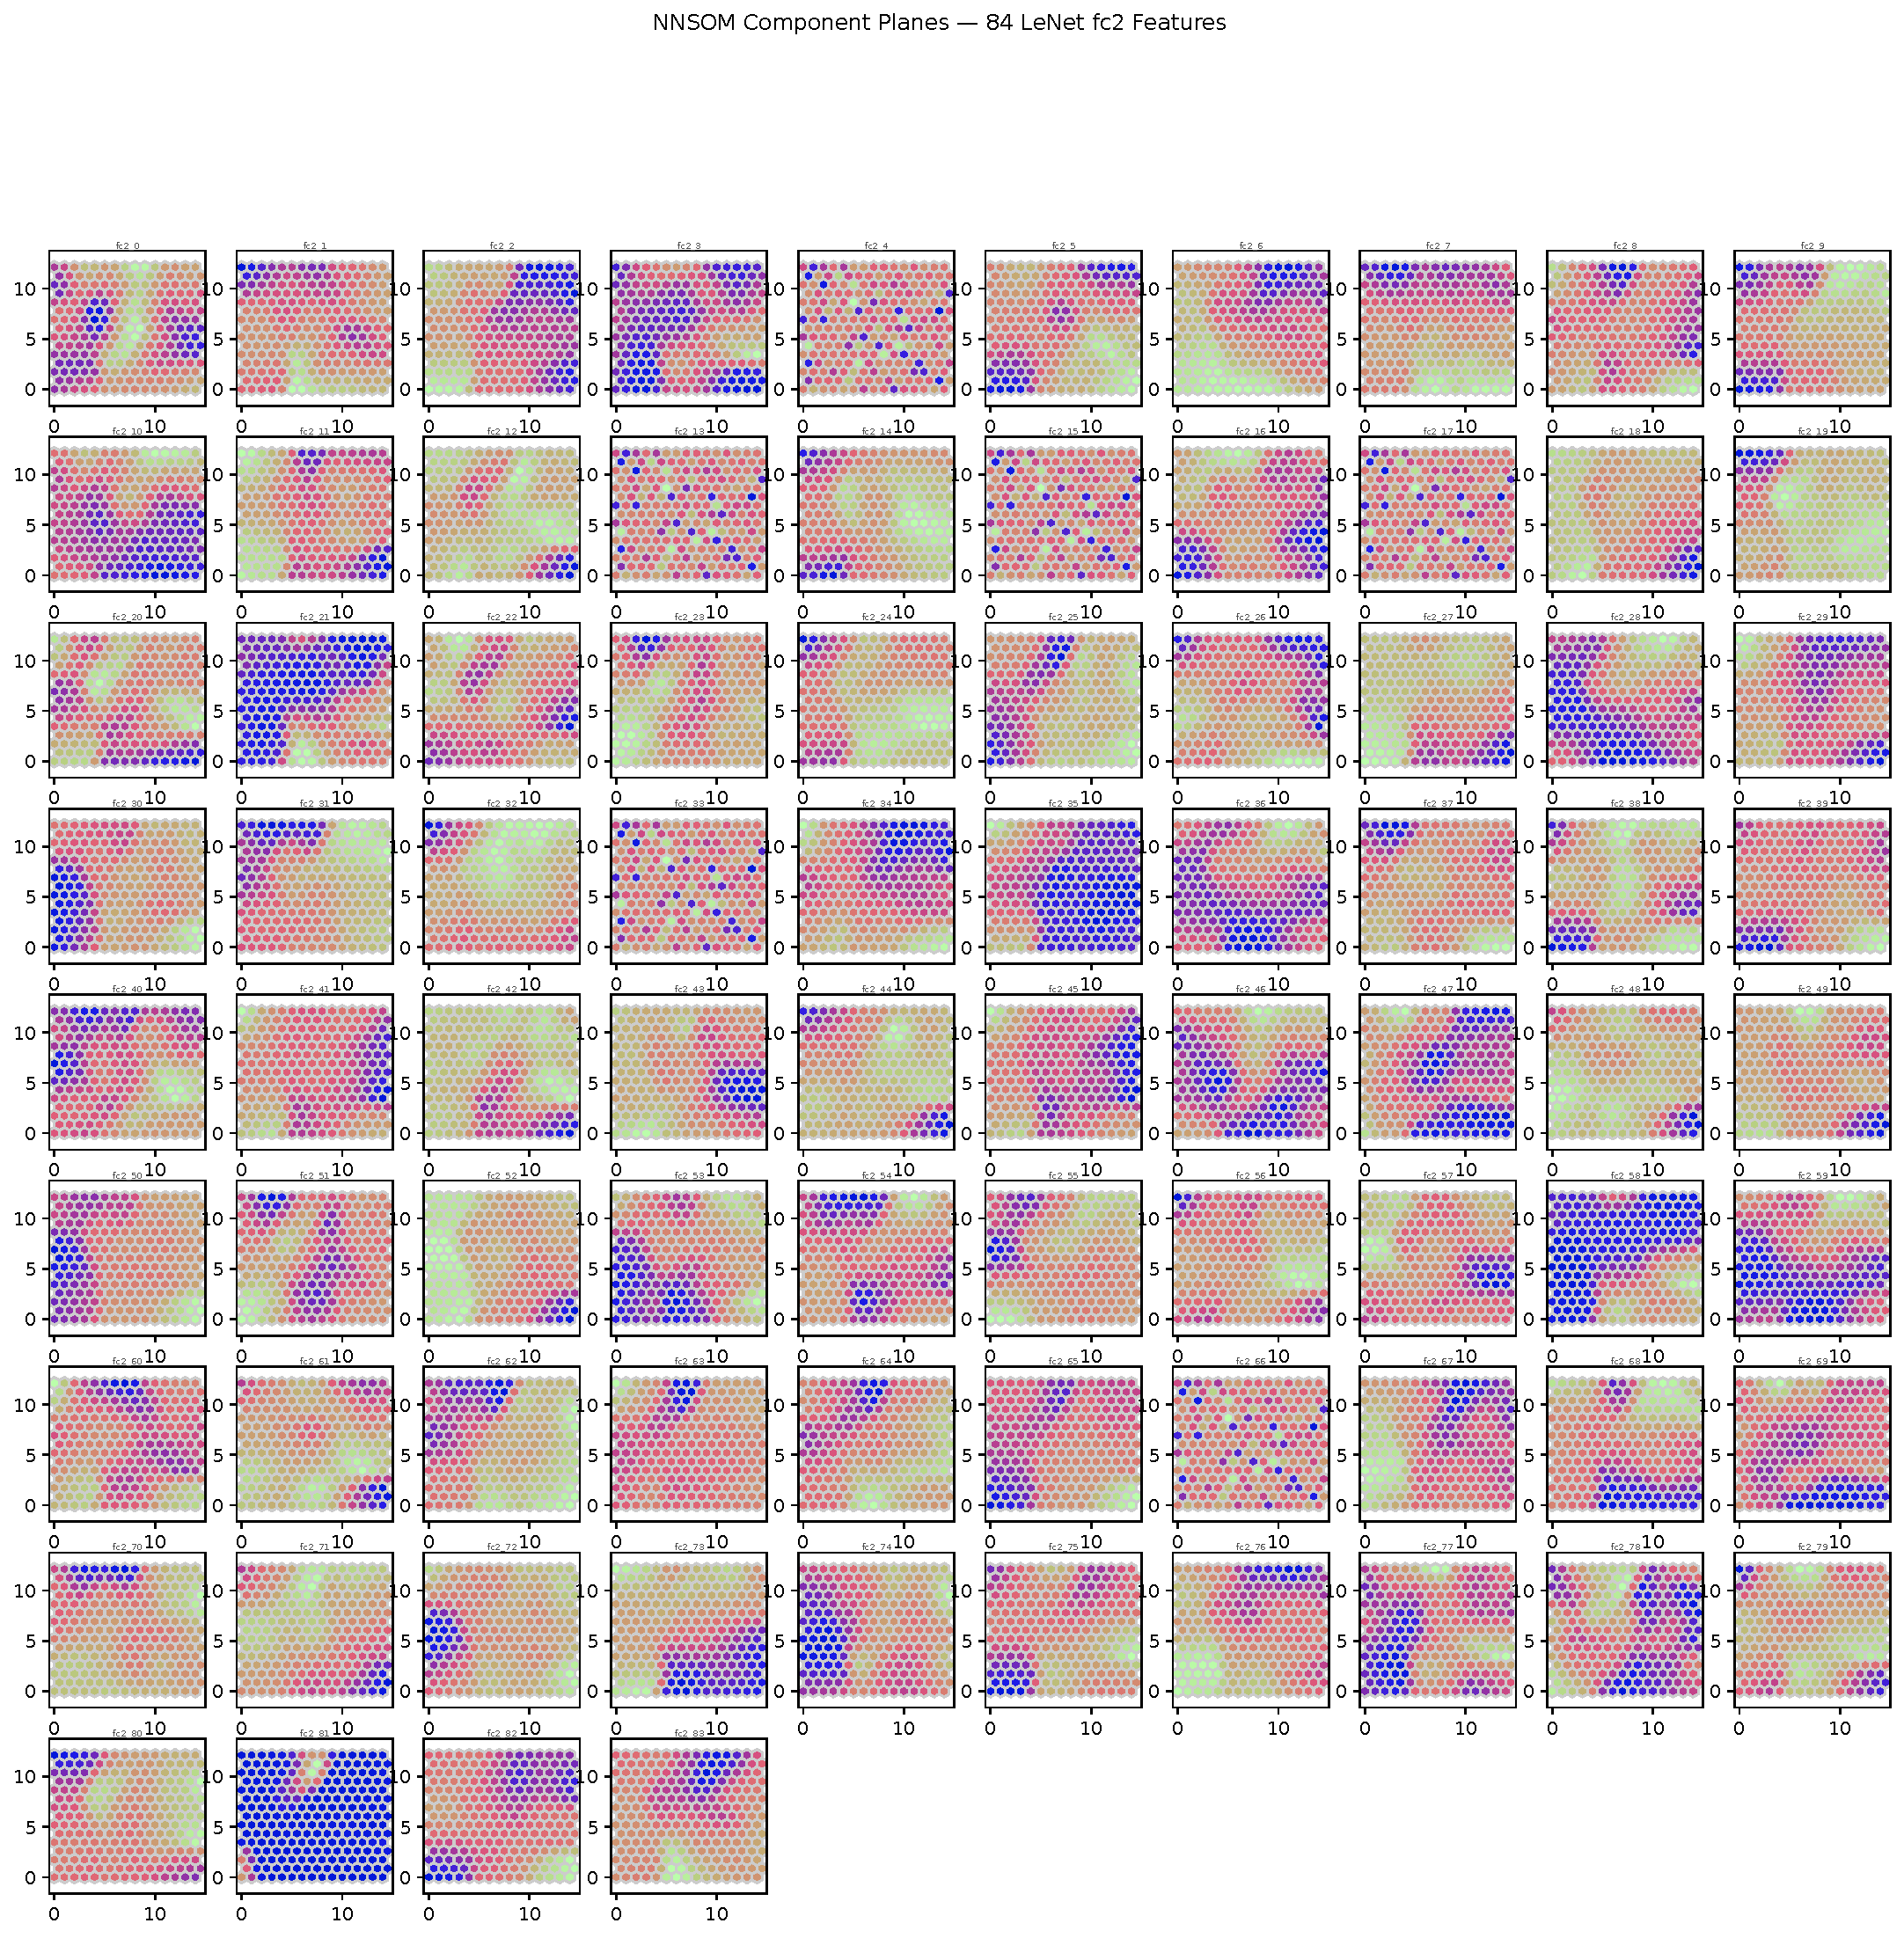
\includegraphics[width=0.80\textwidth]{fig/som_nnsom_training/component_planes/component_planes_all84_nnsom.pdf}
\caption{Component planes of all 84 embedding numbers (one small map each).}
\label{fig:planes}
\end{figure}

\section{Cluster Analysis}\label{sec:cluster}

\begin{itemize}[leftmargin=1.4em, itemsep=2pt]
\item \textbf{Method (same as MNIST).} Every training and validation image is assigned to its best-matching cell. For every cell we count the images of each class (NNSOM's \texttt{cal\_class\_cluster\_intersect}) and compute its most common class, purity and entropy \cite{vesanto2000clustering}. To compare with chance, the class labels are shuffled 1,000 times while every image keeps its cell.

\item \textbf{The classes form regions (Figure~\ref{fig:purity}).} Every class is the most common class in 15 to 29 cells. The weighted purity is 89.33\% on validation images (training: 90.03\%), against 17.3\% (95\% range 17.0--17.7\%) with shuffled labels ($p=0.001$). So the map clearly orders the clothes by class, far beyond chance.

\item \textbf{But many cells are mixed.} Only 73 of the 222 occupied cells hold a single class; 121 have a purity below 95\% and 63 below 80\% (the lowest is 23\%). On MNIST only 44 cells were below 95\%. In the purity map the mixed cells form one large band in the clothing part of the map, while the trouser, bag and footwear regions are almost pure.

\item \textbf{Where confusions happen.} The three most frequent validation confusions, Shirt called T-shirt/top (97), T-shirt/top called Shirt (88) and Pullover called Coat (75), are spread over 24 to 27 cells each. On MNIST each top confusion sat on only 4 or 5 cells. On Fashion-MNIST the confused classes share a whole stretch of the map, not just its edges. Figure~\ref{fig:overlay} shows this: the circled cells of each confusion fill a band across the clothing part of the map.
\end{itemize}

\begin{figure}[H]
\centering
\begin{minipage}[c]{0.46\textwidth}\centering
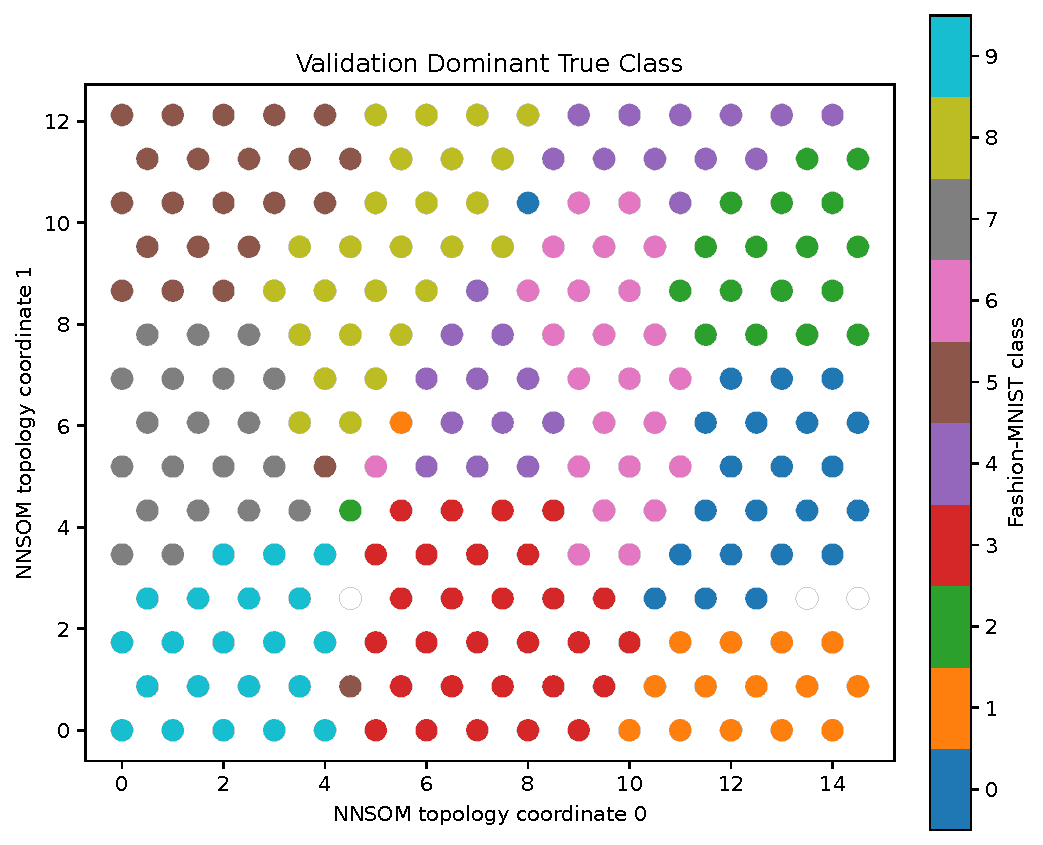
\includegraphics[width=\linewidth,keepaspectratio]{fig/cluster_analysis/analysis_maps/validation_dominant_class.pdf}
\end{minipage}\hfill
\begin{minipage}[c]{0.52\textwidth}\centering
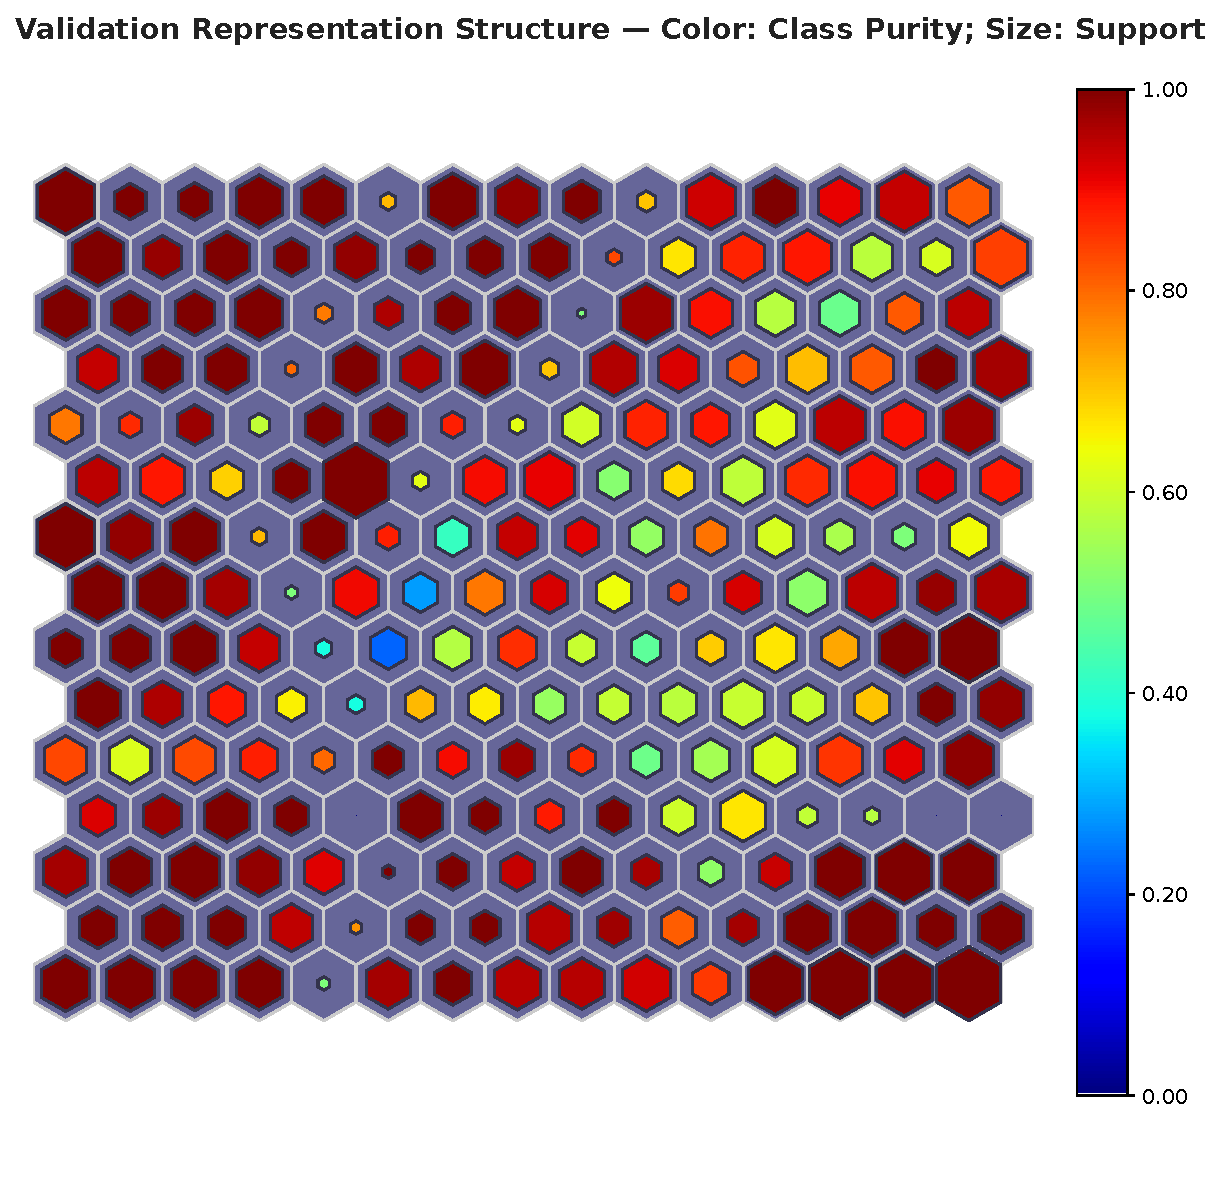
\includegraphics[width=\linewidth,keepaspectratio]{fig/cluster_analysis/analysis_maps/validation_purity_support.pdf}
\end{minipage}
\caption{Left: the most common class of each cell (validation images; 0 T-shirt/top, 1 Trouser, 2 Pullover, 3 Dress, 4 Coat, 5 Sandal, 6 Shirt, 7 Sneaker, 8 Bag, 9 Ankle boot). Footwear (5, 7, 9) sits on the left, bags (8) next to it, and the upper-body garments (0, 2, 4, 6) on the right. Right: purity of each cell (colour) and number of validation images (size). The lower-purity cells form a band where the upper-body garments meet.}
\label{fig:purity}
\end{figure}

\begin{figure}[H]
\centering
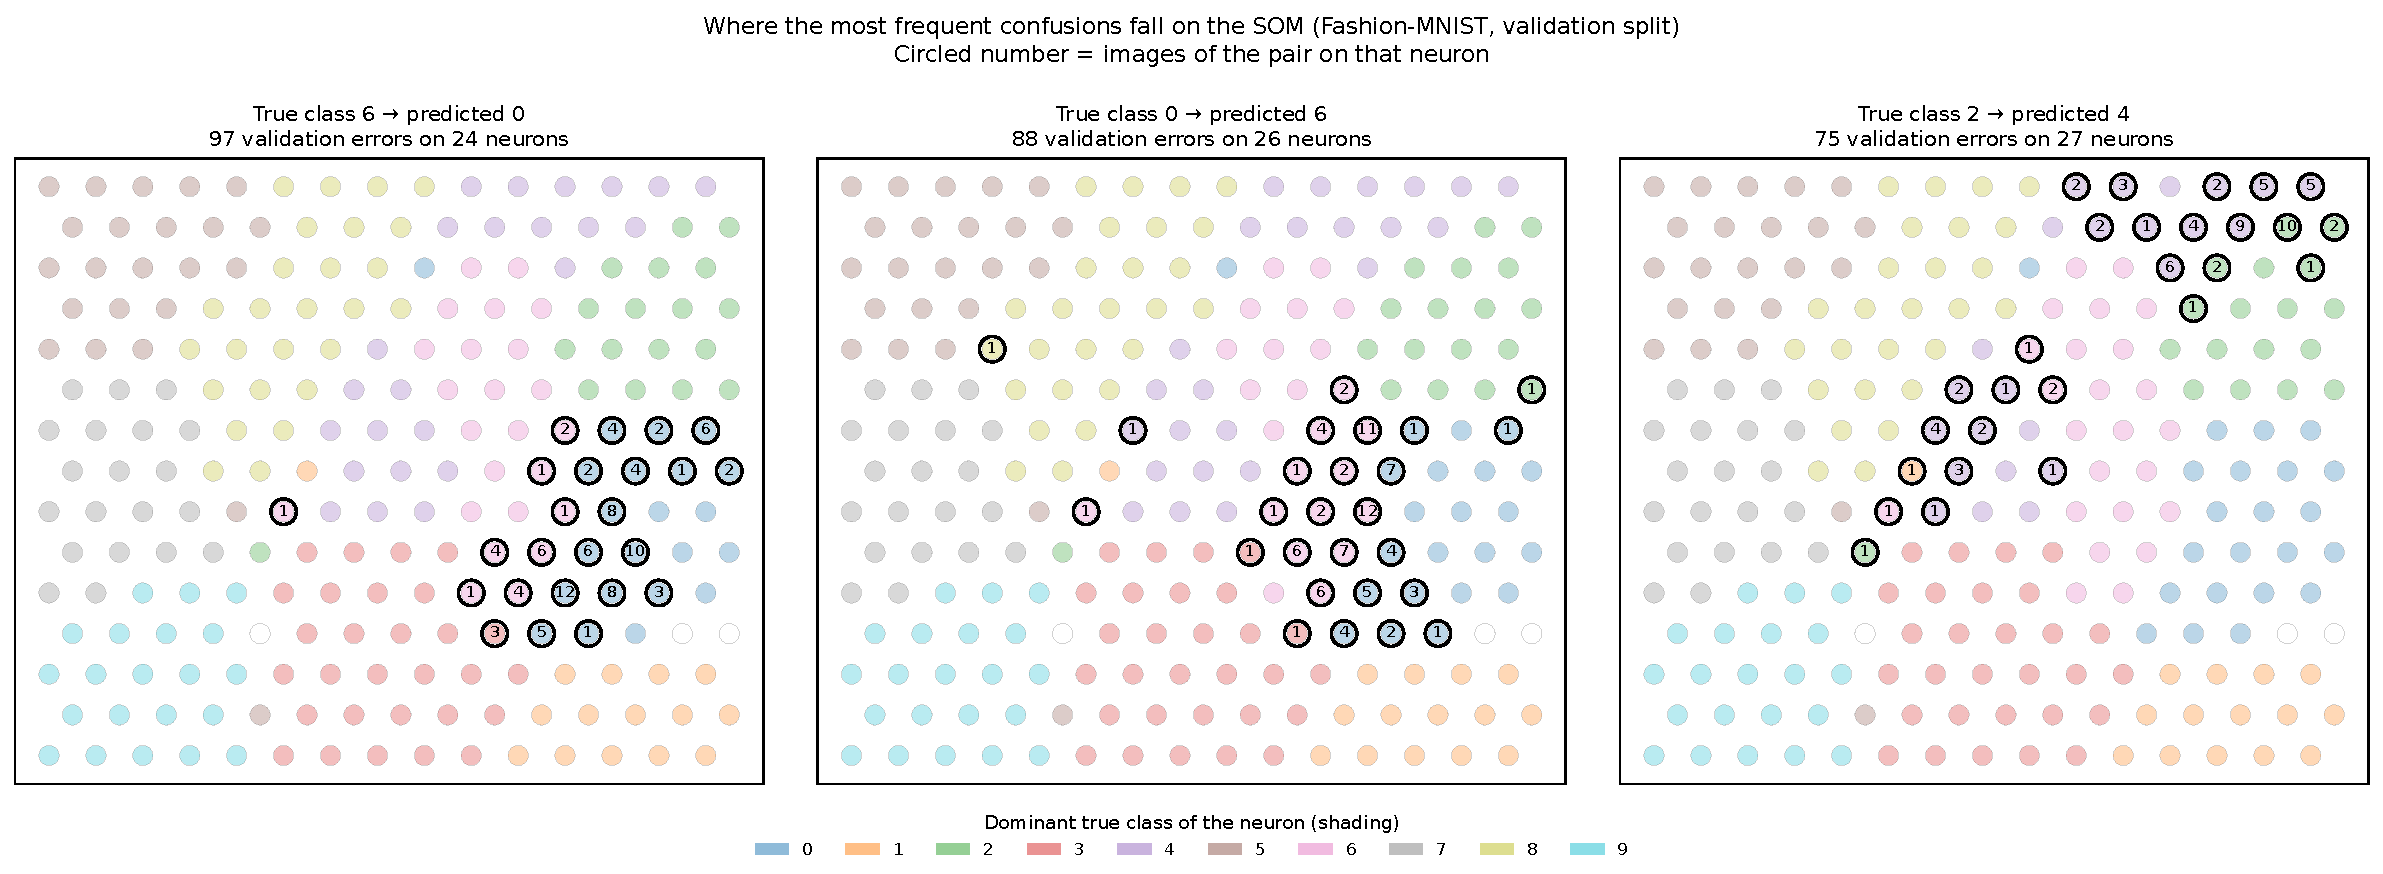
\includegraphics[width=\textwidth]{fig/cluster_analysis/analysis_maps/validation_confusion_overlay.pdf}
\caption{Where the three most frequent confusions fall on the map (validation images): Shirt called T-shirt/top (97 mistakes on 24 cells), T-shirt/top called Shirt (88 on 26 cells), Pullover called Coat (75 on 27 cells). The circled number is how many images of that confusion sit in the cell.}
\label{fig:overlay}
\end{figure}

\section{Error Pattern Analysis}\label{sec:error}

\begin{itemize}[leftmargin=1.4em, itemsep=2pt]
\item \textbf{Correct against wrong.} The network gets 876 of the 10,500 validation images wrong (8.34\%). It is less sure when it is wrong (average confidence 0.686) than when it is right (0.942). Wrong images also sit farther from their cell (average distance 0.994, against 0.840 for correct images).

\item \textbf{Hotspots (Table~\ref{tab:hotspots}).} With the MNIST rule, the 11 cells with the highest Wilson lower bound of their error rate are the hotspots. On the full validation set they hold 4.0\% of the images and 19.7\% of the mistakes (173 of 876). This overstates the effect, because the same images pick the hotspots and count their mistakes. The fair test picks the hotspots on one half of the validation images and counts the mistakes on the other half, 200 times. It gives a concentration ratio of \textbf{3.90} (95\% range 3.23--4.44), against about 1.00 with shuffled mistake labels ($p=0.005$, Table~\ref{tab:robust}).

\item \textbf{What is in the hotspots.} Table~\ref{tab:hotspots} shows that every hotspot mixes upper-body garments: Coat with Shirt or Dress (cells 113, 96), Pullover with Coat (208, 126), Shirt with T-shirt/top (71, 131) or Pullover (145), Dress with Coat (82). Two hotspots (95, 110) hold a little of almost every clothing class. No hotspot is in the footwear or bag regions, although two (95 and 145) hold a few bags. So, unlike MNIST, where hotspots held odd handwriting, the Fashion-MNIST hotspots mark places where whole classes overlap.

\item \textbf{The images in the hotspots (Figure~\ref{fig:samples}), and why they are hard.} We looked at one misclassified image from each hotspot. Our reading, which is a hypothesis and not a tested result:
  \begin{itemize}[leftmargin=1.2em, itemsep=0pt]
  \item \emph{Garments that look alike:} most examples are one upper-body garment called another: T-shirt/top called Shirt (cells 126, 131), Pullover called Shirt, Coat or Dress (110, 208, 113), Coat called Shirt or Dress (96, 82), and a Dress called T-shirt/top (71). At $28\times28$ pixels a collar, buttons or sleeve length are only a few pixels.
  \item \emph{Unusual items:} two bags shaped or patterned like clothing (called Coat in cell 95 and T-shirt/top in cell 145), and one dark, heavily patterned pullover called Sandal (cell 79).
  \item \emph{Often unsure:} the network's confidence in these wrong answers is 0.39 to 0.88, lower than on MNIST, where several hotspot mistakes were made with confidence above 0.97.
  \end{itemize}

\item \textbf{Comparison with simple baselines (Table~\ref{tab:baselines}).} Because the SOM is trained on the network's own embeddings, we checked whether simpler tools find the same pattern, on the same validation embeddings (exploratory, as on MNIST). A k-means grouping with 225 groups finds mistakes as well as the SOM cells (AUROC 0.812 against 0.811). The impurity of the 15 nearest training embeddings does better (0.876), and the network's own confidence (max-softmax \cite{hendrycks2017baseline}) does best (0.906). When every method may flag the same 3.5\% of the images as the SOM's hotspots, the SOM catches 13.7\% of the mistakes, nearest-neighbour impurity 21.1\% and the confidence score 21.9\%. The gap is smaller than on MNIST (18\% against 53\%), because on Fashion-MNIST the network is often wrong without being unsure.

\item \textbf{Overlap regions.} A cell's error rate goes down as its purity goes up (Spearman $-0.946$) and up as its class mix grows ($+0.956$), far beyond chance ($p=0.005$). Both are stronger than on MNIST ($-0.810$ and $+0.816$).

\item \textbf{Other grid sizes (Table~\ref{tab:robust}).} Both findings hold on the 10$\times$10 and 20$\times$20 maps too, with concentration ratios of 3.81 in both cases. The rules for this check are MNIST's, written down before either dataset's check was run.

\item \textbf{Why the ratio is lower than on MNIST (11.1).} A concentration ratio can never be larger than one divided by the overall error rate: about 12 on Fashion-MNIST (8.3\% wrong) but about 114 on MNIST (0.9\% wrong). On MNIST a few mistakes sat in a few small cells, so 5\% of the map could hold a large share of them. On Fashion-MNIST almost a tenth of the images are wrong and they are spread over a whole mixed region, so 11 cells can hold only part of it. The ratio still shows clear clustering; it is not comparable between datasets.
\end{itemize}

\begin{table}[H]
\centering
\renewcommand{\arraystretch}{1.08}
\small
\begin{tabular}{|c|c|c|c|c|l|}
\hline
\textbf{Cell} & \textbf{Images} & \textbf{Wrong} & \textbf{Error} & \textbf{Wilson} & \textbf{Classes in the cell (validation images)} \\ \hline
113 & 36 & 18 & 0.50 & 0.345 & Coat 23, Shirt 7, Pullover 3, Dress 3 \\ \hline
95 & 40 & 19 & 0.48 & 0.329 & Shirt 9, Bag 9, Coat 6, Pullover 5, 3 others \\ \hline
82 & 32 & 15 & 0.47 & 0.309 & Dress 17, Coat 10, Shirt 4, Pullover 1 \\ \hline
79 & 8 & 5 & 0.63 & 0.306 & Pullover 3, Dress 2, 3 others \\ \hline
131 & 41 & 17 & 0.41 & 0.278 & Shirt 25, T-shirt/top 13, Bag 2, Pullover 1 \\ \hline
208 & 31 & 13 & 0.42 & 0.264 & Pullover 19, Coat 12 \\ \hline
145 & 57 & 21 & 0.37 & 0.255 & Shirt 33, Pullover 18, 4 others \\ \hline
110 & 36 & 14 & 0.39 & 0.248 & Trouser 10, Shirt 8, Pullover 6, 3 others \\ \hline
71 & 62 & 22 & 0.35 & 0.247 & T-shirt/top 38, Shirt 19, Dress 5 \\ \hline
96 & 44 & 16 & 0.36 & 0.238 & Coat 25, Dress 7, 4 others \\ \hline
126 & 36 & 13 & 0.36 & 0.225 & Coat 15, Pullover 10, Shirt 7, 3 others \\ \hline
\end{tabular}
\caption{The 11 hotspot cells of the 15$\times$15 map, in rank order (validation images). The overall validation error rate is 0.083.}
\label{tab:hotspots}
\end{table}

\begin{table}[H]
\centering
\renewcommand{\arraystretch}{1.12}
\small
\begin{tabular}{|l|c|c|c|}
\hline
\textbf{Measure (validation images)} & \textbf{10$\times$10} & \textbf{15$\times$15} & \textbf{20$\times$20} \\ \hline
Hotspot cells & 5 & 11 & 20 \\ \hline
Concentration ratio (95\% range) & 3.81 (3.07--4.37) & 3.90 (3.23--4.44) & 3.81 (3.14--4.35) \\ \hline
Chance level (median / 95th percentile) & 1.00 / 1.22 & 1.00 / 1.16 & 1.00 / 1.18 \\ \hline
Spearman, error rate vs.\ purity & $-0.926$ & $-0.946$ & $-0.954$ \\ \hline
Spearman, error rate vs.\ class mix (entropy) & $+0.939$ & $+0.956$ & $+0.954$ \\ \hline
Distance to cell, wrong / correct images & 1.092 / 0.952 & 0.994 / 0.840 & 0.928 / 0.779 \\ \hline
\end{tabular}
\caption{Where the 876 validation mistakes gather, on three grid sizes. Hotspots are picked on one half of the validation images and measured on the other (200 splits); chance comes from 200 shuffles of the mistake labels. All $p=0.005$, the smallest value possible with 200 shuffles.}
\label{tab:robust}
\end{table}

\begin{table}[H]
\centering
\renewcommand{\arraystretch}{1.12}
\footnotesize\setlength{\tabcolsep}{3pt}
\begin{tabular}{|l|c|c|c|c|}
\hline
\textbf{Method} & \textbf{AUROC (95\% range)} & \textbf{Hotspot ratio} & \textbf{Images flagged} & \textbf{Mistakes caught} \\ \hline
SOM cell (15$\times$15) & 0.811 (0.796--0.824) & 3.9 (3.2--4.4) & 3.5\% & 13.7\% \\ \hline
k-means cell (225) & 0.812 (0.805--0.821) & 4.0 (3.7--4.5) & 4.0\% & 15.8\% \\ \hline
15-nearest-neighbour impurity & 0.876 (0.864--0.888) & -- & 3.5\% & 21.1\% \\ \hline
Max-softmax confidence & 0.906 (0.898--0.914) & -- & 3.5\% & 21.9\% \\ \hline
\end{tabular}
\caption{How well each score finds the 876 validation mistakes. For the last two rows the images flagged are set to the SOM's 3.5\% so that the comparison is fair (95\% ranges: 19.2--22.9\% and 19.8--24.1\%). Exploratory. Runs \texttt{error\_pattern\_baselines\_som\_15x15} and \texttt{error\_detector\_budget\_som\_15x15}.}
\label{tab:baselines}
\end{table}

\begin{figure}[H]
\centering
\begin{minipage}[c]{0.50\textwidth}\centering
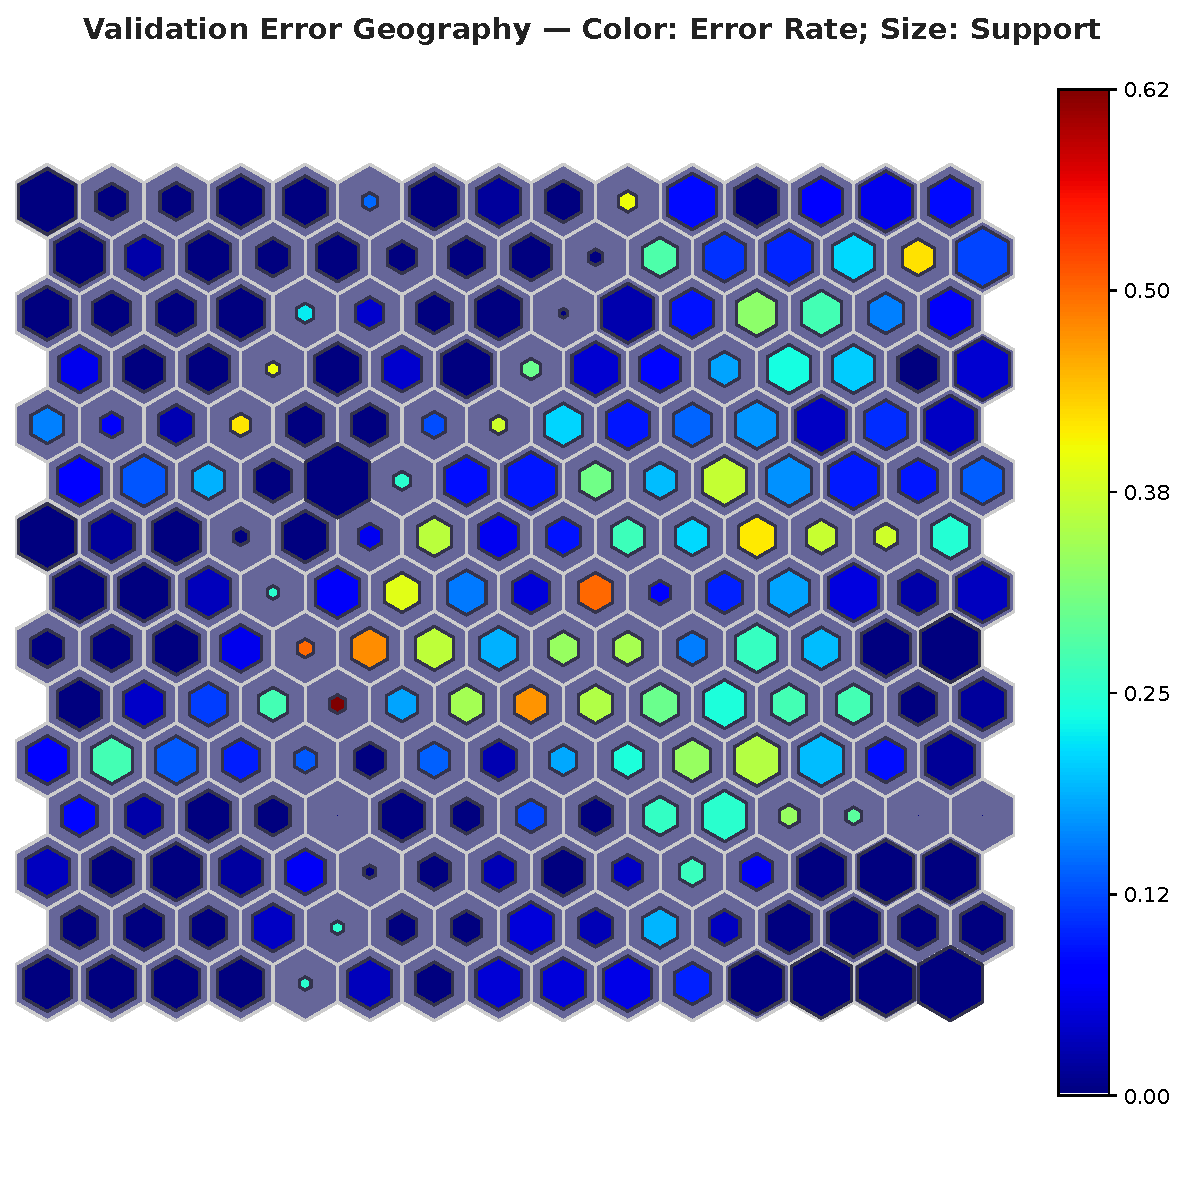
\includegraphics[width=\linewidth,keepaspectratio]{fig/error_pattern_analysis/analysis_maps/validation_error_rate_support.pdf}
\end{minipage}\hfill
\begin{minipage}[c]{0.48\textwidth}\centering
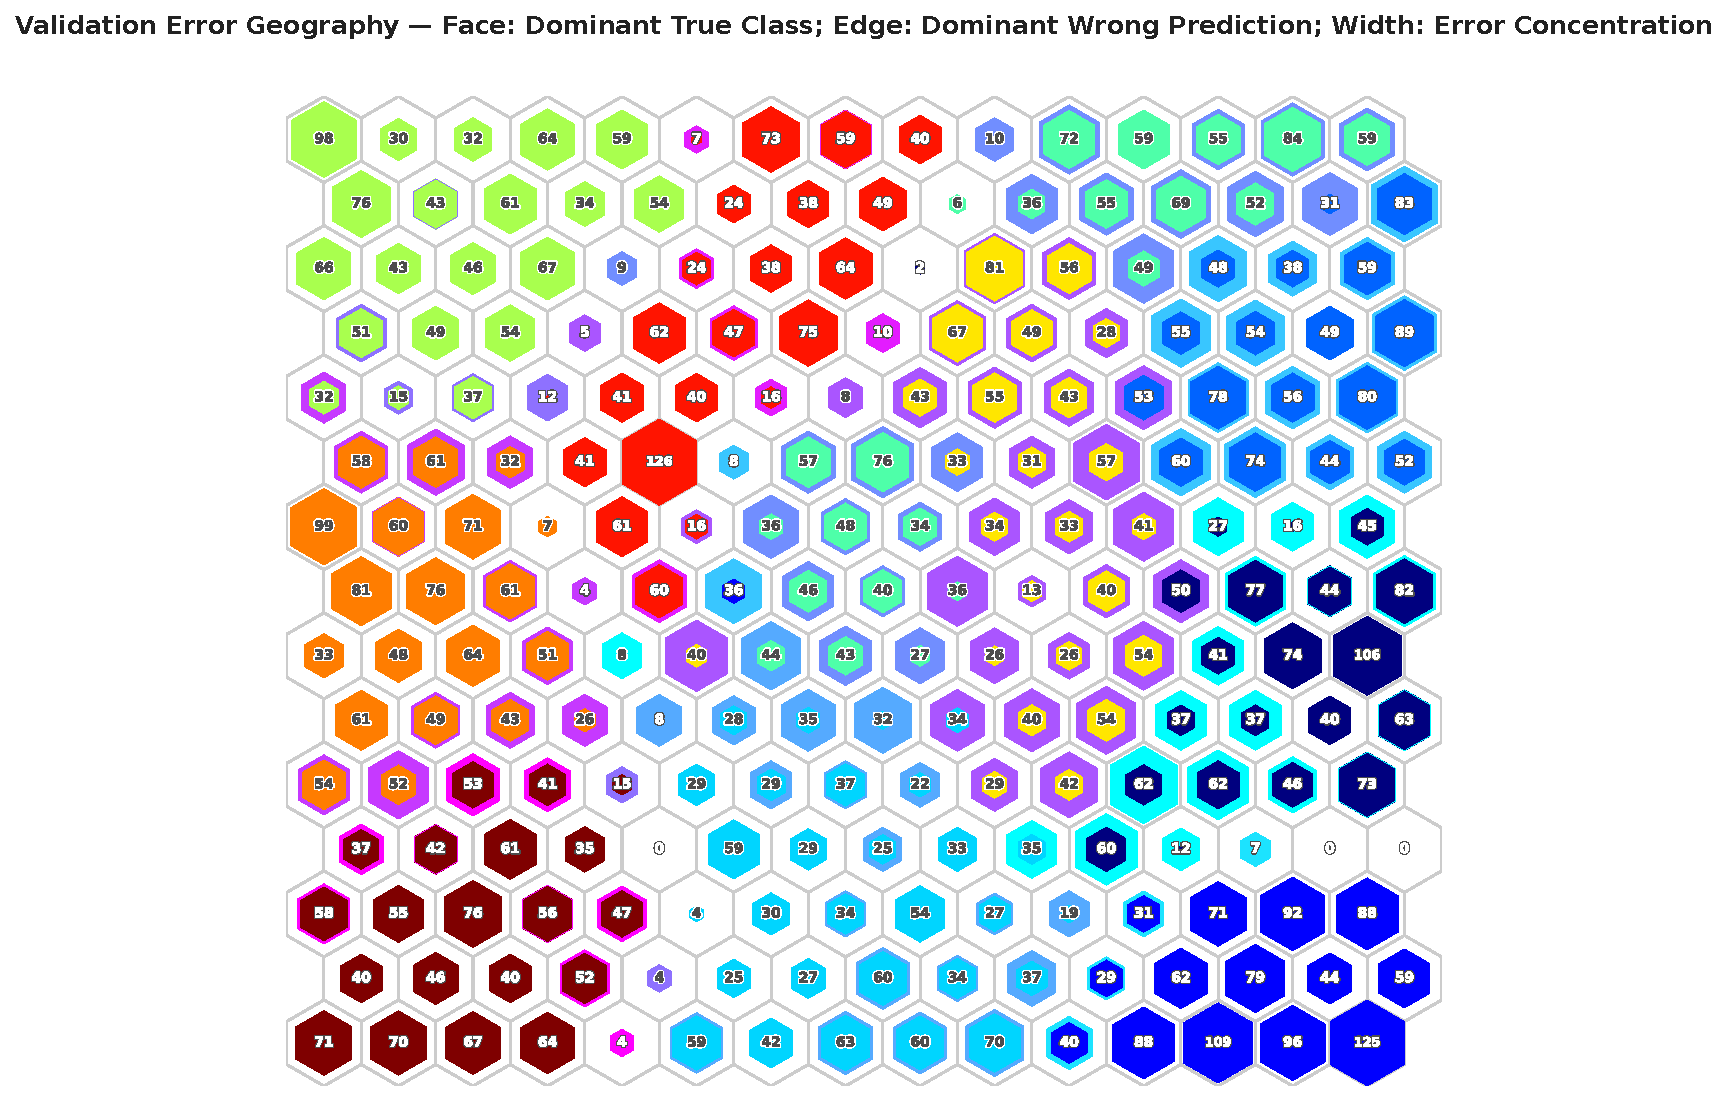
\includegraphics[width=\linewidth,keepaspectratio]{fig/error_pattern_analysis/analysis_maps/validation_complex_error_map.pdf}
\end{minipage}
\caption{Left: error rate of each cell (colour) and number of validation images (size). Right: error map; the fill is the cell's most common true class, the edge colour its most common wrong answer, and the edge width how many mistakes it holds. The mistakes fill the middle band of the map, where the upper-body garments are.}
\label{fig:errormaps}
\end{figure}

\begin{figure}[H]
\centering
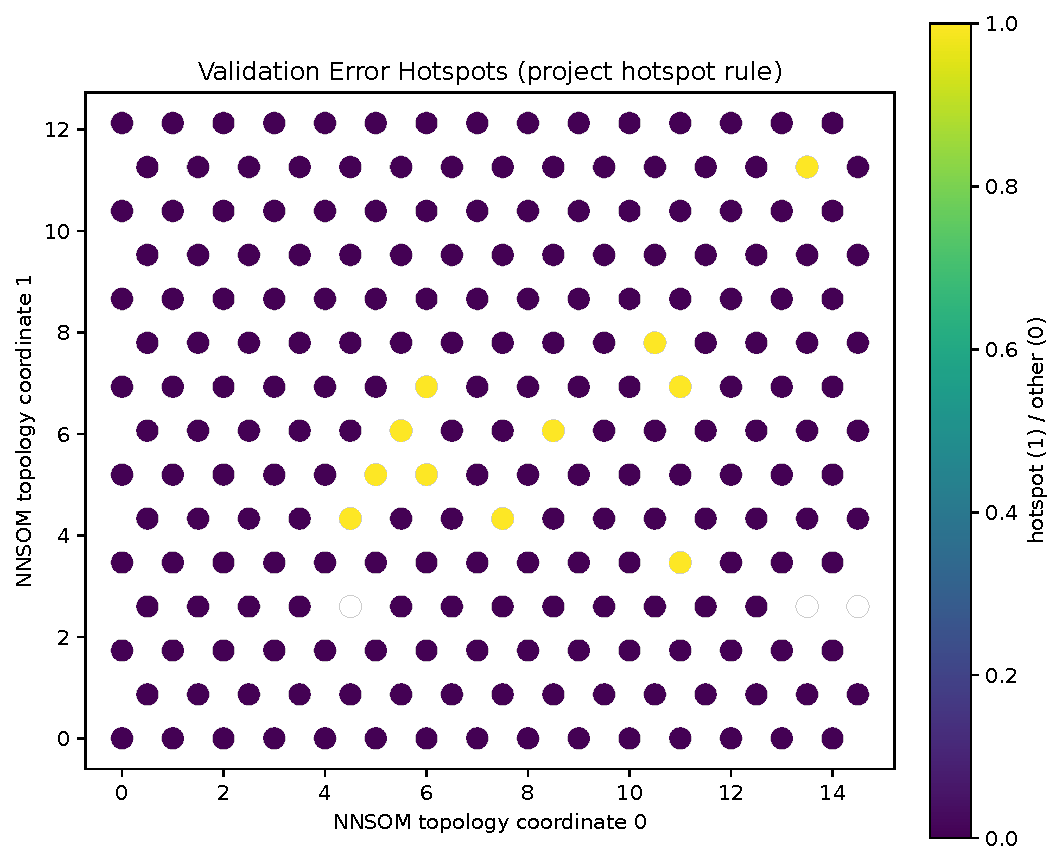
\includegraphics[width=0.50\textwidth,keepaspectratio]{fig/error_pattern_analysis/analysis_maps/validation_hotspot_map.pdf}
\caption{The 11 hotspot cells (yellow). They lie in the clothing part of the map, mostly where the upper-body garment regions meet.}
\label{fig:hotspotmap}
\end{figure}

\begin{figure}[H]
\centering
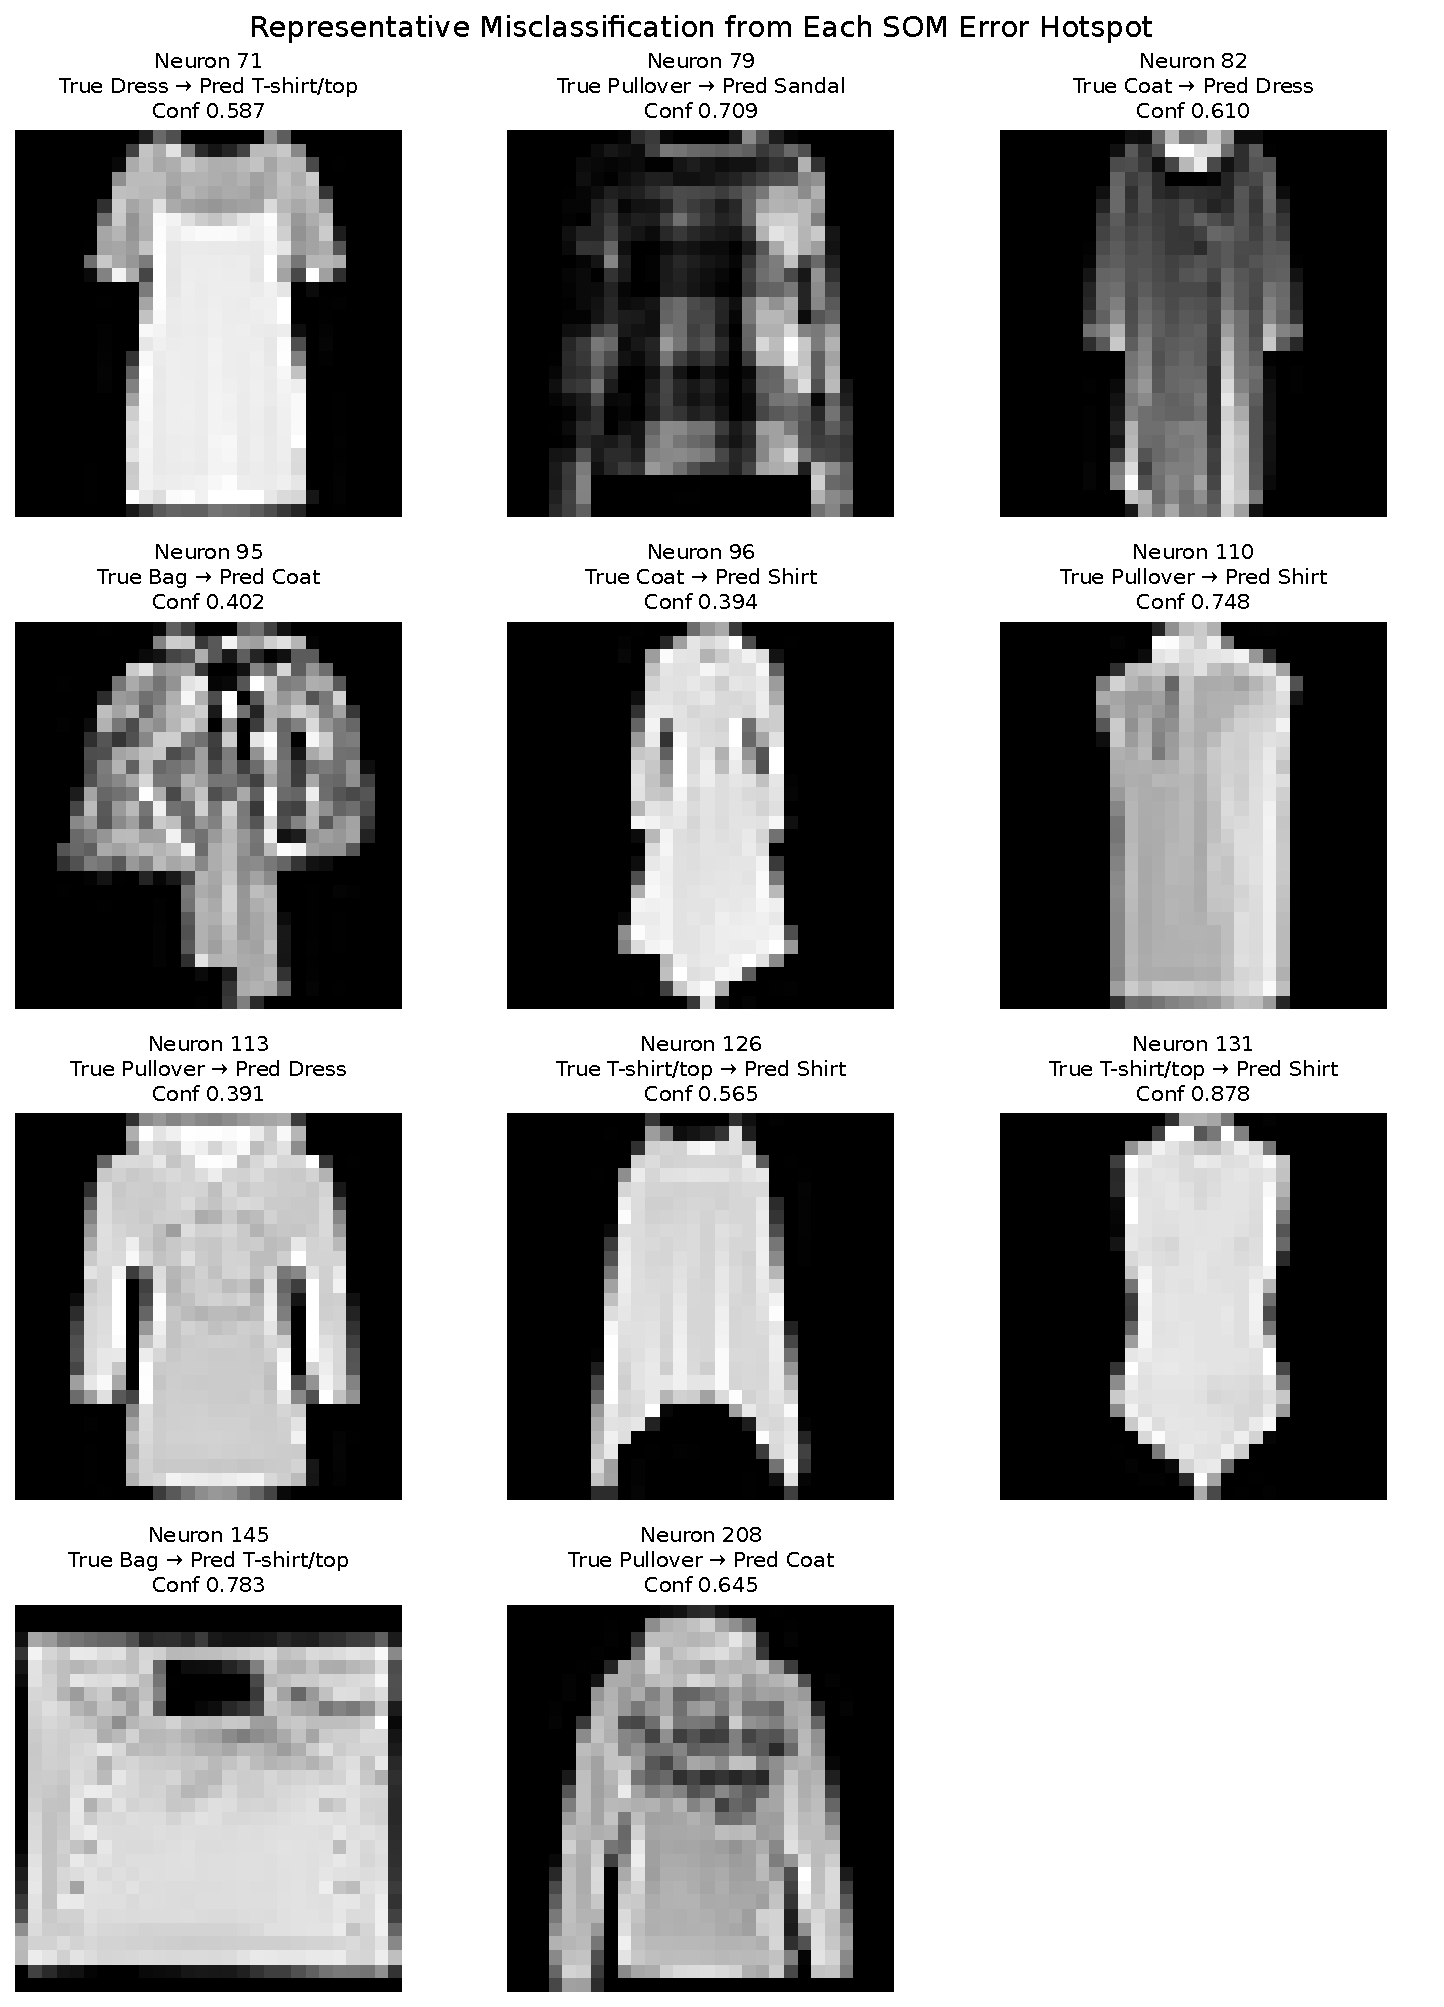
\includegraphics[width=0.62\textwidth,keepaspectratio]{fig/error_pattern_analysis/representative_samples/hotspot_representatives.pdf}
\caption{One misclassified validation image from each of the 11 hotspot cells, with the true class, the network's answer and its confidence.}
\label{fig:samples}
\end{figure}

\section{Feature-Layer Ablation: \texttt{fc1} against \texttt{fc2}}\label{sec:ablation}

The map is trained on the \texttt{fc2} layer (84 numbers). This check asks whether the earlier \texttt{fc1} layer (120 numbers) would give a better map. Both layers of the frozen Phase 1 network are mapped with the same 15$\times$15 recipe and 5 new SOM seeds (1--5), and the two layers are compared seed by seed (95\% $t$-interval over the 5 differences, \texttt{fc1} minus \texttt{fc2}). The statements were fixed in the protocol before any \texttt{fc1} embedding was extracted, and \texttt{fc2} stays the headline layer whatever the result. As a check of the code, the re-extracted \texttt{fc2} embeddings match the Phase 1 ones to within $4\times10^{-6}$.

\begin{table}[H]
\centering
\renewcommand{\arraystretch}{1.12}
\footnotesize\setlength{\tabcolsep}{4pt}
\begin{tabular}{|l|c|c|c|l|}
\hline
\textbf{Measure (validation, mean of 5 seeds)} & \textbf{fc1} & \textbf{fc2} & \textbf{fc1 $-$ fc2 [95\% interval]} & \textbf{Verdict} \\ \hline
L1 (primary): error-cell AUROC & 0.760 & 0.815 & $-0.055$ [$-0.066$, $-0.043$] & fc2 better \\ \hline
L2: weighted purity & 0.842 & 0.890 & $-0.048$ [$-0.051$, $-0.045$] & fc2 better \\ \hline
L3: QE novelty AUROC (SVHN) & 0.902 & 0.815 & $+0.087$ [$+0.027$, $+0.148$] & fc1 better \\ \hline
\multicolumn{5}{|l|}{\textit{Also reported}} \\ \hline
Hotspot error rate & 0.363 & 0.429 & $-0.065$ [$-0.101$, $-0.030$] & \\ \hline
Hotspot share of all mistakes & 0.151 & 0.195 & $-0.045$ [$-0.051$, $-0.038$] & \\ \hline
Topographic error TE1 (\%) & 6.60 & 5.61 & $+1.00$ [$+0.60$, $+1.40$] & \\ \hline
\end{tabular}
\caption{SOMs on the \texttt{fc1} and \texttt{fc2} layers, 5 SOM seeds each. The error-cell AUROC measures how well a cell's error rate predicts the network's mistakes. Run \texttt{feature\_layer\_ablation\_som15x15\_nb11\_ep250\_seeds5}.}
\label{tab:ablation}
\end{table}

\begin{itemize}[leftmargin=1.4em, itemsep=2pt]
  \item \textbf{For error analysis, \texttt{fc2} is better} (L1, L2). Its maps find the network's mistakes better, have purer cells, put more of the mistakes in their hotspots and are better ordered, in every one of the 5 seeds. This supports keeping \texttt{fc2} as the headline layer.
  \item \textbf{For spotting SVHN, \texttt{fc1} is better} (L3, 0.902 against 0.815). The earlier layer still carries more about how an image looks, and SVHN looks very different. The interval is wide because the \texttt{fc2} maps vary a lot by seed (0.766 to 0.884).
  \item \textbf{Seed-to-seed variation.} The five \texttt{fc2} maps give an error-cell AUROC of 0.811 to 0.817 and a purity of 88.8\% to 89.3\%, so these measures hardly depend on the SOM seed; the headline map (seed 42, purity 89.3\%) is typical.
\end{itemize}

\section{Deviations from the plan}

\begin{itemize}[leftmargin=1.4em, itemsep=2pt]
\item \textbf{Test images not mapped.} The project proposal says to assign the training and test images to their cells. As on MNIST, only the training and validation images are mapped, so that the test split stays untouched until the final evaluation in Phase 4.
\item \textbf{No learning rate.} NNSOM's batch rule has no learning rate, so only the grid size, the starting radius and the number of epochs were set, all copied from MNIST.
\item \textbf{Steps run late.} The error-pattern baselines, the same-budget comparison and the grid comparison were run after the Phase 3 results were known, because the pipeline did not run them by default (the grid comparison code was not yet in the repository). Their rules are MNIST's, unchanged, and none of them reads any Phase 3 result. The cluster and error-map figures were made with the other Phase 2 runs but were tracked with DVC only later; nothing was re-run. All of this is recorded in the Fashion-MNIST deviation log.
\end{itemize}

\section{Leakage Control}

\begin{itemize}
  \item The SOM was trained on the 49,000 training embeddings. The scaler that maps the embeddings to $[-1,1]$ was fitted on the training embeddings only and applied unchanged to the validation embeddings.
  \item All Phase 2 numbers use training and validation images. The test embeddings are never loaded: the SOM, cluster and error runs record \texttt{test\_evaluated: false}.
  \item The grid comparison follows MNIST's pre-registered design and decision rule unchanged, on validation images only. The baseline comparison is exploratory, as on MNIST.
  \item The SOM recipe, the hotspot rule, the number of splits and shuffles and all seeds were copied from MNIST and written in the Fashion-MNIST protocol before any Fashion-MNIST data was loaded. The Optuna check was also fixed in advance, and its result could not change the headline map.
  \item Every run records the SHA-256 of its inputs (the Phase 1 embeddings and the SOM model), and a finished run is never overwritten.
  \item The CNN used the same validation split to choose its best epoch, so validation is not completely untouched by model development.
\end{itemize}

\section{Limitations}\label{sec:open}

All Phase 2 steps of the protocol have been run. Limitations: one CNN and one SOM seed for the headline results (the ablation shows that the SOM seed changes purity and error-cell AUROC very little); the SOM recipe is MNIST's and was not tuned for Fashion-MNIST, although the Optuna check found no better setting; the baseline comparison is exploratory; the explanations of the hotspot images come from looking at eleven images and are hypotheses.

\section{Discussion}
\begin{itemize}[leftmargin=1.4em, itemsep=2pt]
\item \textbf{The map is a good picture of what the CNN has learned.} It separates footwear, trousers and bags cleanly and puts the upper-body garments in one large, mixed region, which matches the classes the network confuses.
\item \textbf{The CNN's mistakes are not random.} They gather in hotspots about four times more than chance, on all three grid sizes, and a cell's error rate follows its class mix very closely ($\rho\approx-0.95$).
\item \textbf{The kind of failure differs from MNIST.} On MNIST the hotspots were a few small cells with unusual handwriting. On Fashion-MNIST they lie inside a broad overlap between whole classes. So the map's value here is to show \emph{which group of classes} the network cannot separate, not single odd images.
\item \textbf{The right layer depends on the job.} \texttt{fc2} gives the better map of the network's mistakes; \texttt{fc1} separates SVHN better. Since this phase is about mistakes, \texttt{fc2} is the right choice here, but Phase 3's far-novelty results would likely be stronger on \texttt{fc1}.
\item \textbf{The SOM explains, it does not detect best.} A plain k-means grouping finds mistakes as well as the SOM cells, and nearest-neighbour impurity and the network's confidence do better. The gap is smaller than on MNIST, but the conclusion is the same: the SOM's value is in showing \emph{where} the mistakes are and which classes they involve.
\end{itemize}

\section{Conclusion and Next Phase}

\begin{itemize}[leftmargin=1.4em, itemsep=2pt]
\item With the MNIST recipe unchanged, a 15$\times$15 SOM orders the Fashion-MNIST embeddings by class (89.3\% purity against 17.3\% by chance), with one large mixed region for the upper-body garments.
\item The fair grid comparison supports 15$\times$15 over 20$\times$20; a k-means grouping finds mistakes as well as the SOM, and the network's confidence does better.
\item The \texttt{fc2} layer gives a better map of the mistakes than \texttt{fc1} in all 5 SOM seeds.
\item The network's 876 validation mistakes gather in 11 hotspot cells (3.9 times their fair share, held-out test) where classes mix, and this holds on 10$\times$10 and 20$\times$20 maps.
\item \textbf{Next phase.} Phase 3 uses the same frozen map to test whether images far from their cell (large quantization error) are unlike the training data; misclassified images are already farther away (0.994 against 0.840). Phase 4 uses the hotspots to choose images for retraining, where Fashion-MNIST's many mistakes leave far more room for gains than MNIST did.
\end{itemize}

\printbibliography[title={References}]

\end{document}
